% ── Section 2: Data and case-study setting ────────────────
\section{Data and Case-Study Setting}
\label{sec:data}

\subsection{Study site and monitoring stations}

Tongoy Bay is monitored by two CEAZAMET stations \citep{ceazamet_network,ceazamet_btg_station}
(Figure~\ref{fig:site-context}): the Tongoy buoy
(BTG), a floating platform (lat~$-30.275$\textdegree{}, lon~$-71.562$\textdegree{})
carrying the in-situ chlorophyll (channel BTGCLF) and dissolved-oxygen (channel BTGOXD2) sensors
used in this report, and PLV, a coastal meteorological mast at Punta Lengua de Vaca
($\sim$15~km away), sited at a known regional
upwelling centre \citep{moraga2001plv} and providing wind, solar radiation, humidity, and
pressure. Both provide hourly observations from 2015 to 2026. Satellite and reanalysis products (chlorophyll, sea-surface temperature, wind stress, and
ocean currents) are extracted over a fixed regional box around the Tongoy coordinate and
used as external predictors in both case studies (Table~\ref{tab:data_sources}; full
extraction detail in Appendix~\ref{sec:appendix_repro}).

\begin{table}[htbp]
\centering
\caption{Main external predictor products. Product-level provenance and citations are given in
Appendix~\ref{app:data_products}.}
\label{tab:data_sources}
\small
\begin{tabular}{p{4cm}p{6cm}p{1.6cm}p{2.5cm}}
\toprule
Product & Scientific role & Coverage & Resolution \\
\midrule
GlobColour L4 \chl{} & Regional surface-biology proxy & 90\% & $\sim$4~km, daily \\
MUR SST & Thermal tracer / surface state & 98\% & $\sim$1~km, daily \\
CMEMS winds & Regional wind forcing for upwelling & 90\% & $\sim$25~km, hourly \\
PLV station & Local atmospheric forcing & 76\% & point, hourly \\
GLORYS12 currents & Shelf transport / advection predictors & $>$99\% & $\sim$8~km, daily \\
\bottomrule
\end{tabular}
\end{table}

Table~\ref{tab:data_sources} is easier to interpret in the physical setting of the Tongoy coast.
This part of northern-central Chile belongs to the Humboldt upwelling system, where
equatorward alongshore winds can drive offshore Ekman transport in the surface layer.
The resulting nearshore divergence is compensated by the upward movement of colder,
nutrient-rich subsurface water onto the shelf and into the coastal zone
\citep{kampf2016upwelling, montecino2009humboldt}. Figure~\ref{fig:upwelling_schematic}
shows this process schematically for the Tongoy Bay setting.

\begin{figure}[htbp]
  \centering
  
\includegraphics[width=0.75\textwidth]{figures/fig_upwelling_schematic.png}
  \caption{Conceptual schematic of the upwelling setting relevant to Tongoy Bay.}
  \label{fig:upwelling_schematic}
\end{figure}

This process motivates the external predictors used later in the benchmark.
Wind from PLV and reanalysis represents the mechanical forcing of upwelling,
sea-surface temperature (SST) acts as a thermal tracer of recently upwelled water and
surface stratification, satellite chlorophyll provides a biological proxy, and
ocean-current fields represent advection, exchange, and retention on the shelf.

The same predictor families are plausible for both case
studies, as their interaction can explain part of the physical process, but their usefulness will be established empirically in the benchmark.

\subsection{Case Study 1: chlorophyll-\textit{a} target, distribution, and missingness}
\label{sec:chl_target}

\noindent
\begin{minipage}[t]{0.57\textwidth}
The chlorophyll reconstruction target is the daily mean in-situ \chl{} from the Tongoy buoy
(BTG) fluorometer channel BTGCLF, expressed in mg~m\textsuperscript{$-3$} and computed from
hourly observations. A day is eligible only if at least 18 hourly values are valid
(coverage $\geq 75\%$); otherwise it is excluded from the target and treated as missing.
The eligible daily distribution is strongly right-skewed, with intermittent
high-concentration days (Figure~\ref{fig:chl_distribution}). For this reason, all models
are fitted on $\log_{10}(\texttt{chl\_mean})$, while physical-unit values are retained for
interpretation.

\medskip

Over 3988 days (2015-07-01 to 2026-05-31), 3012 (75.5\%) are eligible and 976
are missing, forming 128 real gaps (Figure~\ref{fig:chl_target_and_gaps}). Most gaps are
brief interruptions, but the record also contains a 256-day gap from 2020-02-11 to
2020-10-23. This very long gap spans three seasons and
is treated only as an illustrative reconstruction scenario because no validation is available for such long gaps.
\end{minipage}
\hfill
\begin{minipage}[t]{0.39\textwidth}
\vspace{-0.6em}
\centering
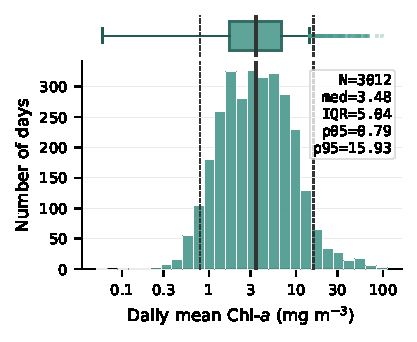
\includegraphics[width=\linewidth]{figures/fig_chl_distribution.pdf}
\captionsetup{justification=raggedright,singlelinecheck=false,font=footnotesize}
\captionof{figure}{Distribution of eligible daily chlorophyll-\textit{a}. The solid line marks
the median; dashed lines mark p05 and p95.}
\label{fig:chl_distribution}
\end{minipage}

\vspace{0.8em}

\begin{figure}[htbp]
  \centering
  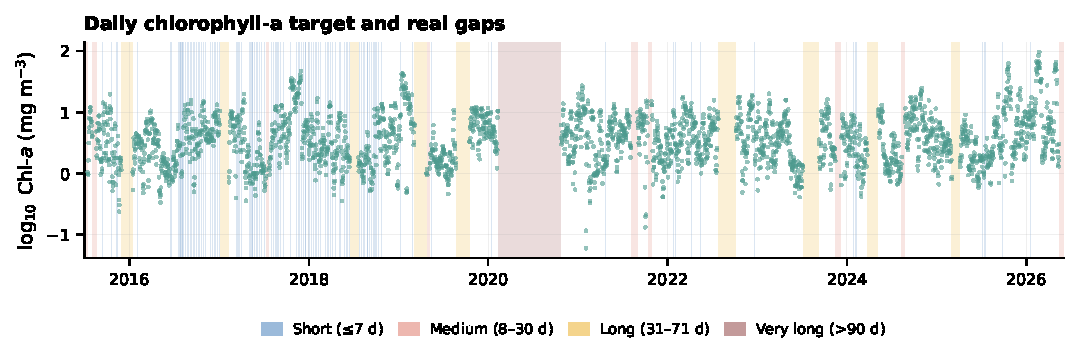
\includegraphics[width=0.96\textwidth]{figures/fig_chl_target_and_gaps.pdf}
  \caption{Observed daily chlorophyll-\textit{a} and real-gap structure at Tongoy buoy (BTG).}
  \label{fig:chl_target_and_gaps}
\end{figure}

\subsection{Case Study 2: dissolved oxygen target, distribution, and missingness}
\label{sec:oxygen_data}

\noindent
\begin{minipage}[t]{0.57\textwidth}
The dissolved oxygen reconstruction target is the daily mean oxygen concentration from the
Tongoy buoy (BTG) sensor channel BTGOXD2, expressed in mg/L and computed from hourly
observations. The same daily eligibility rule is used as for chlorophyll: a day enters the
target only if at least 18 hourly values are valid. Across eligible days, the distribution
has median 6.429~mg/L, with p05 2.818~mg/L and p95 8.802~mg/L, and includes both low and
high tails (Figure~\ref{fig:oxygen_distribution}).

\medskip

Over the same 3988-day span (2015-07-01 to 2026-05-31), 2880 days (72.2\%) are eligible
and 1108 are missing or ineligible, forming 125 real gaps
(Figure~\ref{fig:oxygen_target_and_gaps}). The three largest are a 256-day gap shared with
chlorophyll from 2020-02-11 to 2020-10-23, a 161-day oxygen-specific gap from 2025-02-08
to 2025-07-18, and a 71-day gap from 2022-07-27 to 2022-10-05. 
\end{minipage}
\hfill
\begin{minipage}[t]{0.39\textwidth}
\vspace{-0.6em}
\centering
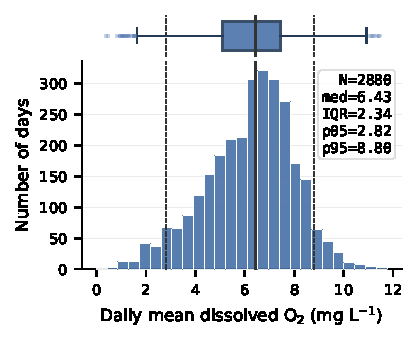
\includegraphics[width=\linewidth]{figures/fig_oxygen_distribution.pdf}
\captionsetup{justification=raggedright,singlelinecheck=false,font=footnotesize}
\captionof{figure}{Distribution of eligible daily dissolved oxygen. The solid line marks
the median; dashed lines mark p05 and p95.}
\label{fig:oxygen_distribution}
\end{minipage}

\vspace{0.8em}

\begin{figure}[htbp]
  \centering
  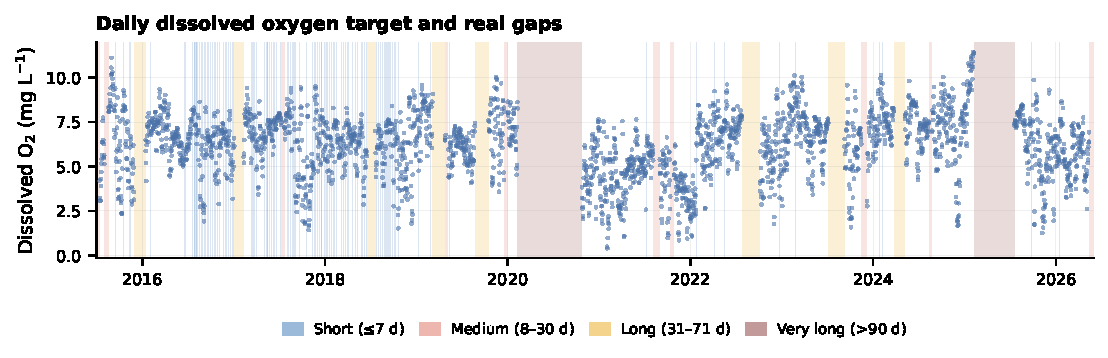
\includegraphics[width=0.96\textwidth]{figures/fig_oxygen_target_and_gaps.pdf}
  \caption{Observed daily dissolved oxygen and real-gap structure at Tongoy buoy (BTG).}
  \label{fig:oxygen_target_and_gaps}
\end{figure}

\subsection{Predictor channels and feature construction}
\label{sec:predictors}

The data products introduced above are converted into predictor channels before modelling.
These channels summarize five types of information: seasonality, target history outside the
hidden gap, satellite biological signal, atmospheric/upwelling forcing, and ocean
current/transport conditions (Table~\ref{tab:predictor_families}). Feature construction is both
temporal and spatial. Temporal features include lags, rolling means, cumulative indices, and
pre-/post-gap boundary summaries. Spatial features summarize gridded products around Tongoy, for example through nearest-cell values, regional means, local variability, or
coastal gradients. This avoids reducing every external product to a single nearest pixel.

\begin{table}[htbp]
\centering
\caption{Predictor channels and representative feature constructions. Full feature lists are
given in Appendix~\ref{sec:appendix_repro}.}
\label{tab:predictor_families}
\small
\renewcommand{\arraystretch}{1.15}
\begin{tabularx}{\textwidth}{P{3.0cm}Y Y}
\toprule
Channel & What is encoded & Representative features \\
\midrule
Calendar / seasonality
& Position within the annual cycle.
& Month; $\sin$/$\cos$ day-of-year terms. \\

Target history / gap-edge context
& Observed target behaviour immediately outside the hidden gap.
& Last pre-gap value; 7-d pre-gap mean and slope; first post-gap value; post-gap mean;
edge-to-edge change and slope. \\

Satellite biological proxy
& Regional surface chlorophyll information from satellite products.
& Nearby or regional $\log_{10}$ \chl{}; local box means; chlorophyll anomaly; valid-pixel
fraction; patchiness metrics. \\

Atmospheric / upwelling forcing
& Wind, radiation, SST, and upwelling-related surface forcing.
& PLV solar radiation; wind speed; cumulative upwelling index; rolling SST; recent SST
cooling. \\

Ocean current / transport
& Advection, exchange, and retention conditions over the regional extraction box.
& Surface current speed; alongshore current component;
Okubo--Weiss-type transport summaries. \\
\bottomrule
\end{tabularx}
\end{table}

The representation of these channels depends on the model family. Tabular models see one
feature vector per target day, so temporal and spatial context must be encoded explicitly in
the columns. This is why the tabular feature set contains rolling windows, lags, cumulative
forcing indices, regional summaries, and gap-edge statistics. TS-ICL instead receives
time-indexed target and covariate sequences over a context window. Its covariates can still be
engineered channels, but they are supplied as sequences rather than collapsed into a single
row. Therefore, the same scientific information families can be used across model families
without requiring the exact same feature representation.